\documentclass[12pt]{article}
\usepackage[hidelinks]{hyperref}    
\usepackage[all]{hypcap}
\usepackage{amssymb}
\usepackage{amsmath}
\usepackage{xcolor}
\usepackage{graphicx}
\graphicspath{{../images/}}
\title{\textbf{Analisi Matematica\\Non numerabilità di $\mathbb{R}$ e la radice aritmetica}}
\date{26 settembre 2024}
\author{Andrea Malvezzi}
\begin{document}
\maketitle
\pagebreak
\tableofcontents
\pagebreak
\section{L'insieme $\mathbb{R}$ è numerabile?}
Per capire se $\mathbb{R}$ sia numerabile o meno, è sufficiente studiare l'intervallo in $\mathbb{R}$ $[0,1[$.
\subsection{Dimostrazione per assurdo} \label{dim:non_numerabilità_R}
Supponiamo per assurdo che esista una funzione suriettiva definita da $\mathbb{N}$ a $[0,1[$:
\[f: \mathbb{N} \rightarrow [0,1[\]
\begin{center}
    quindi:
\end{center}
\[f(n) \in [0,1[, \text{ con } f(n) = 0, x_{n_0}, x_{n_1}, \dots\]
Mostriamo ora che esiste un numero \textbf{reale} (che chiameremo $r$) $\in [0,1[$ t.c.:
\[f(n) \not= r, \forall n \in \mathbb{N}\]
Per farlo, costruiamo il nostro numero $r$ tramite un procedimento diagonale (da \textit{Cantor}):
\begin{gather*}
    r := 0, r_0, r_1, r_2, \dots \\
    r_j = \begin{cases}
        5 \text{ se } x_{n_n} \not= 5\\
        6 \text{ se } x_{n_n} = 5
    \end{cases}
\end{gather*}
\begin{center}
    Dove $x_{n_n}$ equivale ai termini con indici uguali tra loro di una matrice costruita basandosi sui risultati di $f(n)$, quindi:
\end{center}
\begin{gather*}
    f(0) = 0, \colorbox{yellow}{$x_{0_0}$}, x_{0_1}, x_{0_2}, \dots \\
    f(1) = 0, x_{1_0}, \colorbox{yellow}{$x_{1_1}$}, x_{1_2}, \dots \\
    f(2) = 0, x_{2_0}, x_{2_1}, \colorbox{yellow}{$x_{2_2}$}, \dots \\
    \dots\\
    r = 0, x_{0_0}, x_{1_1}, x_{2_2}
\end{gather*}
Quindi: $f: \mathbb{N} \rightarrow [0,1[$ non è suriettiva. Per assurdo quindi si sa che $\mathbb{R}$ non è numerabile.
\pagebreak
\subsubsection{Esempio}
A seguire un esempio di quanto appena dimostrato:
\begin{figure}[!htb]
    \centering
    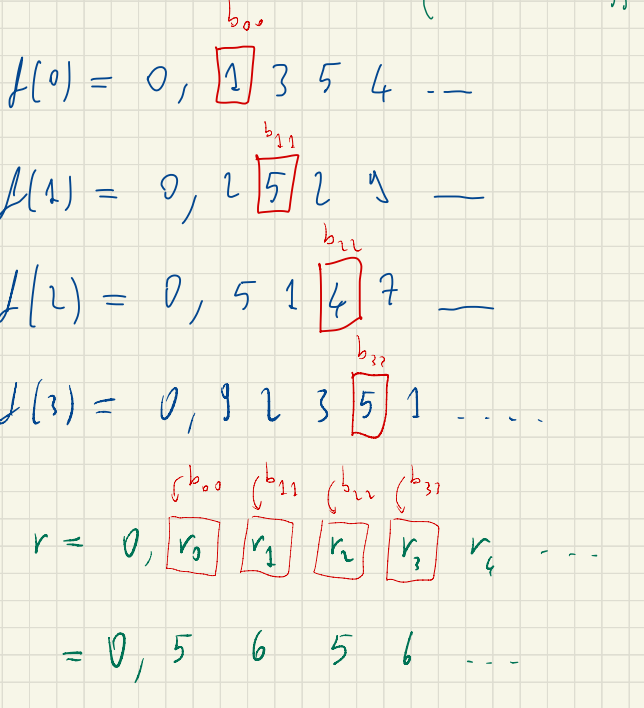
\includegraphics[width=1\textwidth, height=.9\textheight,keepaspectratio]{lezione_4/dim_numerab_r.PNG} % essenzialmente resiza l'immagine
    \begin{center}
        \caption{\label{fig:dim_numerab_r_example}Avendo $r_n$ diverso da $b_{n_n} \forall n \in \mathbb{N}$ allora $r \not= f(n) \forall n \in \mathbb{N}$.} % label fuori da caption spesso non va, mettilo dentro
    \end{center}
\end{figure}
\section{La radice}
Ora che si è passati in $\mathbb{R}$ si può parlare di estrazione della radice di un numero:
\subsection{Teorema}
\begin{equation}
    \forall r \in \mathbb{R_+}, \forall n \in \mathbb{N} - \{0\}, \exists ! b \in \mathbb{R_+} : b^n = r \label{teo:estrazione_radice}
\end{equation}
Dove $b$ si dice \textbf{radice aritmetica n-sima} di $r$ e si scrive $\sqrt[n]{r} := b$.\\
Inoltre, $b \geq 0$. Perciò, ad esempio:
\[\sqrt{4} = 2, \text{ non } -2\]
\end{document}